%--------------------------------------------------------------------------------
%----------------------------------------------------------------------
\section{Features}\label{sec:features}
Knowledge of the features of GreenMirror is imperative when using the application. The two parts GreenMirror is composed of and their usage is first described in \cref{sec:features;sub:clientserver}. The way a model is interpreted is then elaborated upon in \cref{sec:features;sub:nodrel}, followed by a description of an integral part of the visualizations in \cref{sec:features;sub:placement}: node placement. Further possibilities are presented by discussing all currently available commands in \cref{sec:features;sub:commands}. \Cref{sec:features;sub:log,sec:features;sub:gridbuilder} briefly expand upon two auxiliary functionalities: the log and the \lstinline{GridBuilder} class, respectively.
%--------------------------------------------------------------------------------
\subsection{Client and server}\label{sec:features;sub:clientserver}
The GreenMirror application is divided into two distinct components: the client and the server. The client interprets the user's model and translates it into commands. The server performs the actual visualization on the basis of these commands. Due to this decoupling, the framework is more maintainable and extensible and can thus be easily linked to other components or component versions.
\par Both components have to be executed using command line options. For the client to run, it needs a server to be available. To start the server, only one option has to be provided: the port. Use, for example, the option \lstinline{--port=81} to run the server on port 81. The \lstinline{--verbose} option can be added to enable verbose output to the log and \lstinline{--help} to show all available command line options.
\par The client has three required options: \lstinline{--host}, \lstinline{--model} and \lstinline{--trace}. If a GreenMirror server is running local on port 81, the first option would look like \lstinline{--host=127.0.0.1:81}. To initialize a model using a Groovy script (which is currently the only supported model initializer), use \lstinline{--model=groovyscript:<groovyfile>} and to select a trace using the file selector (which is currently the only supported trace selector), use \lstinline{--trace=file:<tracefile>}. \lstinline{<*file>} should, of course, be replaced with the corresponding file names. Similar to the server, \lstinline{--verbose} and \lstinline{--help} can also be used with the client. For more details, see \cref{sec:design;sub:generalwf,sec:design;sub:detailedwf,sec:design;sub:interface}.
%--------------------------------------------------------------------------------
\subsection{Nodes and relations}\label{sec:features;sub:nodrel}
Tools such as GROOVE \cite{rensink2004} use \emph{nodes} and \emph{edges} to define their model. This terminology can not simply be copied, because the definition and usage of an edge is slightly different than the equivalent entity used in GreenMirror. GreenMirror uses \emph{nodes} and directional \emph{relations} to define the model. State-transitions consist of adding and removing nodes, altering the appearance of nodes and changing relations between nodes. \\
Node properties include a type, a name, labels and an appearance wrapper, all of which are optional. When the node is added to the model, it receives an internal identification number; "ID" for short. The user does not have to interact with this ID in any way. Nodes also store their relations with other nodes. \\
Relations are always directional, going from "node A" to "node B". All relations have a name, a placement, a rigidity and a temporary appearance for node A, of which the latter lasts for the duration of the relation. These properties are optional, although it is recommended to always specify a name. There are two kinds of relations: placement relations, indicating that node A has a placement relative to node B on the visualizer, and non-placement relations, where the placement is set to \lstinline{NONE}. The rigidity property can only be set for placement relations. When set to true it indicates that node A should follow when node B moves on the visualizer. If the rigidity is set to false, the placement is only calculated and applied when the relation is created: it won't be maintained when node B moves.
\par Each GreenMirror node that has a visual appearance needs to store and track the properties of its FX. This is internally done using implementations of the abstract \lstinline{FxWrapper} class. The FX type can only be defined once for every GreenMirror node. The currently supported FX types are:
\begin{itemize}
\item rectangle;
\item circle;
\item text; and
\item image (with a local or remote source).
\end{itemize}
\par Per FX type, certain properties can be set only initially and some can also be set or changed after the node's FX initialization. Due to the nature of GreenMirror, all properties of the latter type must be animatable. The \texttt{opacity} property, for example, is animatable by default by the JavaFX library. The \texttt{width} of a rectangle, on the other hand, is not animatable by default. GreenMirror includes animation support for some properties such as \texttt{width} so these properties can be changed during state-transitions. GreenMirror also supports the animation of some discrete properties, such as the \texttt{text} property of the text FX type. This is done by using a fast fade-out on the JavaFX node, changing the property and then using a fast fade-in. Support for additional FX types and FX type properties can be easily added to the framework. See \cref{sec:design;sub:fxwrapper,app:ext;sub:fxwrapper,app:ext;sub:fxpropertywrapper}.
%--------------------------------------------------------------------------------
\subsection{Node placement}\label{sec:features;sub:placement}
Placements are an important aspect of the visualization of nodes and their relations. They provide a level of abstraction and let the user worry rather about the model than about the actual coordinates of nodes on the visualizer. Placement relations between nodes indicate that one node of the relation, node A, is placed in a specific respect to the other node of the relation, node B. There are currently several extensions of the abstract \lstinline{Placement} class implemented which are described below and are illustrated in \cref{fig:placements}. Every instance of \lstinline{Placement} also has an optional position relative to the placement. For example: if a node A has an edge top placement with relative position \lstinline{(0, -20)} on node B, node A is placed 20 pixels above (and centred on) the edge of node B.
\begin{description}
\item[\texttt{Corner*Placement}] A placement on any of the corners of a JavaFX node: top left, top right, bottom right or bottom left.
\item[\texttt{Edge*Placement}]  A centred placement on any of the edges of a JavaFX node: top, right, bottom or left.
\item[\texttt{MiddlePlacement}] A placement in the exact middle of a JavaFX node.
\item[\texttt{EdgePlacement}]   A placement on the edge of a JavaFX node, according to a specified angle. An angle of zero degrees is the equivalent an edge top placement, and an angle of 90 degrees (positive) is the equivalent of an edge right placement. 
\item[\texttt{CustomPlacement}] A placement where only the relative position data is used to determine the coordinates. The relative position data is relative to the coordinates calculated for the \lstinline{MiddlePlacement}.
\item[\texttt{RandomPlacement}] A random placement on a JavaFX node. Upon receiving this placement data, the server replaces this with a \lstinline{CustomPlacement} where the relative position is set to the calculated, relative coordinates of the \lstinline{RandomPlacement}. This is done so the random coordinates aren't recalculated every time node B moves (in the case of a rigid placement relation).
\item[\texttt{NoPlacement}] The default for a relation.
\end{description}
\begin{figure}[h]
  \centering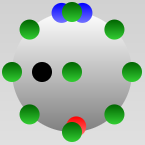
\includegraphics{images/placements}
  \caption{an example available placements on a circle FX node. The green circles have a corner* (or at least, what would have been the corner), edge* or middle placement, the blue ones an edge placement with -10 and 10 degrees, the black one a custom placement with relative position \lstinline{(-10, 0)} and the red one a random placement.}
  \label{fig:placements}
\end{figure}
%--------------------------------------------------------------------------------
\subsection{Commands}\label{sec:features;sub:commands}
In the current version of GreenMirror, communication between the client and the server is one way: all supported commands are meant to be sent from the client to the server. With the information in this section and \cref{sec:design;sub:interchange}, one can develop a completely new client or server that can work with the current version of GreenMirror. For a better overview, the commands have been divided into \cref{tab:commands_vis,tab:commands_model}: the first is about commands relating to the visualizer and the handling of state-transitions, the second is about changes in the model. In the tables, the command name is in the upper left corner, the parameters, their type and their description on the right and the command description underneath those. This section is meant to give an overview of the currently available commands used within GreenMirror: it is not as detailed as the JavaDoc documentation that is available on the repository of this project.
\begin{longtable}{ |l|l r| }
\caption{commands pertaining to the visualizer and the handling of state-transitions}\label{tab:commands_vis}
\\ \hline \multirow{2}{*}{\textbf{Initialization}}
   & \texttt{width} & integer 
\\ & \multicolumn{2}{|l|}{The width of the visualizer window.} 
\\ \cline{2-3} & \texttt{height} & integer
\\ & \multicolumn{2}{|l|}{The height of the visualizer window.}
\\ \cline{2-3} & \texttt{defaultAnimationDuration} & double
\\ & \multicolumn{2}{|l|}{The default time animations will take to complete.}
\\ \cline{2-3} & \texttt{rotateRigidlyRelatedNodesRigidly} & boolean
\\ & \multicolumn{2}{|l|}{\parbox[t]{10.3cm}{Whether the "A" node of a rigid relation should rotate rigidly when the "B" node is rotated.\Bstrut}}
\\ \cline{2-3} \multicolumn{3}{|l|}{\parbox[t]{14.1cm}{\vspace{5px}The initialization command initializes and opens the visualizer with the passed parameters. This should come \emph{before} any command pertaining to the model.\vspace{10px}}}
%--------------------
\\ \hline \pagebreak \hline \multirow{2}{*}{\textbf{SetAnimationDuration}}
   & \texttt{duration} & double
\\\nopagebreak[4] & \multicolumn{2}{|l|}{The duration of all following animations, in milliseconds.}
\\\nopagebreak[4] \cline{2-3} \multicolumn{3}{|l|}{\parbox[t]{14.1cm}{\vspace{5px}This sets the duration of all atomic animations. For example: if the animation duration is set to 1000 milliseconds and five animations will be played sequentially, the total animation duration is 5000 milliseconds.\vspace{10px}}}
%--------------------
\\ \hline\hline \multirow{2}{*}{\textbf{Flush}}
   & \texttt{delay} & double
\\ & \multicolumn{2}{|l|}{The delay that is added after the previous animation, in milliseconds.}
\\ \cline{2-3} \multicolumn{3}{|l|}{\parbox[t]{14.1cm}{\vspace{5px}By default, all animations resulting from one state-transition are played parallel to each other. This command creates a new queue: the set of parallel animations created after this command are played after the set of previously created animations. Optionally, a delay can be added between the previous and upcoming set of animations. Also see \cref{sec:design;sub:states}. \vspace{10px}}}
%--------------------
\\ \hline\hline \multicolumn{3}{|l|}{\multirow{2}{*}{\textbf{EndTransition}}}
\\ \multicolumn{3}{|l|}{\parbox[t]{14.1cm}{\vspace{5px} This command signals the server that the state-transition has ended. \vspace{10px}}}
%--------------------
\\ \hline\hline \multicolumn{3}{|l|}{\multirow{2}{*}{\textbf{StartVisualization}}}
\\ \multicolumn{3}{|l|}{\parbox[t]{14.1cm}{\vspace{5px} The command that tells the server that the visualizations may start. The current version of this server handles this by transitioning to the first state. \vspace{10px}}}
%--------------------
\\ \hline\hline \multicolumn{3}{|l|}{\multirow{2}{*}{\textbf{ExitVisualizer}}}
\\ \multicolumn{3}{|l|}{\parbox[t]{14.1cm}{\vspace{5px} This command communicates to the server that the visualizer should exit. In this version of GreenMirror, the client sends this command if a fatal error is encountered in the user's model. \vspace{10px}}}
\\\hline\end{longtable}
%-*-*-*-*-*-**-*--*-*--*-**--**-*--**-*-*-*--**-*--*
\begin{longtable}{ |l|l r| }
\caption{commands pertaining to the user's model}\label{tab:commands_model}
%--------------------
\\\hline \multirow{2}{*}{\textbf{AddNode}}
   & \texttt{id} & integer 
\\ & \multicolumn{2}{|l|}{The unique, internal ID of the GreenMirror node.} 
\\ \cline{2-3} & \texttt{identifier} & string
\\ & \multicolumn{2}{|l|}{The identifier of the GreenMirror node: the user-defined type and name.}
\\ \cline{2-3} \multicolumn{3}{|l|}{\parbox[t]{14.1cm}{\vspace{5px} This signals that a node has been added to the user's model. The visualizer doesn't have to do anything yet: the FX is yet to be defined at this point. \vspace{10px}}}
%--------------------
\\ \hline\hline \multirow{2}{*}{\textbf{AddRelation}}
   & \texttt{name} & string 
\\ & \multicolumn{2}{|l|}{The name of the relation.} 
\\ \cline{2-3} & \texttt{nodeA} & integer
\\ & \multicolumn{2}{|l|}{The internal ID of node A.}
\\ \cline{2-3} & \texttt{nodeB} & integer
\\ & \multicolumn{2}{|l|}{The internal ID of node B.}
\\ \cline{2-3} & \texttt{placement} & string
\\ & \multicolumn{2}{|l|}{The placement data of node A on node B.}
\\ \cline{2-3} & \texttt{rigid} & boolean
\\ & \multicolumn{2}{|l|}{Whether the relation is rigid or not.}
\\ \cline{2-3} & \texttt{tempFX} & FxWrapper
\\ & \multicolumn{2}{|l|}{The temporary FX of node A.}
\\ \cline{2-3} \multicolumn{3}{|l|}{\parbox[t]{14.1cm}{\vspace{5px} This indicates that a relation has been added between a node "A" and a node "B". If \texttt{placement} is set, the server should handle this. The same goes for \texttt{tempFX}. \vspace{10px}}}
%--------------------
\\ \hline\hline \multirow{2}{*}{\textbf{RemoveNode}}
   & \texttt{id} & integer 
\\ & \multicolumn{2}{|l|}{The internal node ID.} 
\\ \cline{2-3} \multicolumn{3}{|l|}{\parbox[t]{14.1cm}{\vspace{5px} This commands signals that a GreenMirror node has been removed from the user's model. Consequently, all relations have also been removed. \vspace{10px}}}
%--------------------
\\ \hline\hline \multirow{2}{*}{\textbf{RemoveRelation}}
   & \texttt{id} & string
\\ & \multicolumn{2}{|l|}{The unique ID of the relation.} 
\\ \cline{2-3} & \texttt{nodeA} & integer
\\ & \multicolumn{2}{|l|}{The internal ID of node A.} 
\\ \cline{2-3} \multicolumn{3}{|p{14.1cm}|}{\vspace{5px} This commands signals that a relation has been removed. The server should also handle restoring the FX of node A in the case a temporary FX was set. \vspace{10px}}
%--------------------
\\ \hline\hline \multirow{2}{*}{\textbf{SetNodeFX}}
   & \texttt{id} & integer
\\ & \multicolumn{2}{|l|}{The internal ID of the GreenMirror node.} 
\\ \cline{2-3} & \texttt{fx} & FxWrapper
\\ & \multicolumn{2}{|l|}{The FX values.} 
\\ \cline{2-3} \multicolumn{3}{|p{14.1cm}|}{\vspace{5px}This commands communicates with what properties and values the FX of a node should be set. The \texttt{fx} parameter can include all properties that can be set, initially or otherwise (see \cref{sec:features;sub:nodrel}).\vspace{10px}}
%--------------------
\\ \hline\hline \multirow{2}{*}{\textbf{ChangeNodeFX}}
   & \texttt{id} & integer
\\ & \multicolumn{2}{|l|}{The internal ID of the GreenMirror node.} 
\\ \cline{2-3} & \texttt{fx} & FxWrapper
\\ & \multicolumn{2}{|l|}{The new FX values.} 
\\ \cline{2-3} \multicolumn{3}{|p{14.1cm}|}{\vspace{5px} This commands indicates that the FX of a GreenMirror node has been changed. The \texttt{fx} parameter can include only animatable properties (see \cref{sec:features;sub:nodrel}). \vspace{10px}}
\\\hline\end{longtable}
%--------------------------------------------------------------------------------
\subsection{Log}\label{sec:features;sub:log}
It is assumed that any stakeholder working with the tool wants as much data and information as possible about what is happening. GreenMirror uses a static \lstinline{Log} class that accepts any implementation of \lstinline{PrintStream}. During runtime both the client and the server send data and information to their respective log sinks. A time stamp that is accurate to the millisecond is included with each entry, so performance can also be analysed. The client uses \lstinline{System.out} as its log sink, seeing as it does not have a graphical user interface. The server uses \lstinline{System.out} and, as it does have a graphical user interface, GreenMirror's \lstinline{WindowLogger} implementation (depicted in \cref{fig:log}). As was briefly mentioned in \cref{sec:features;sub:clientserver}, a verbose option can be enabled which results in the log being filled with more raw data.
\begin{figure}[h]
  \centering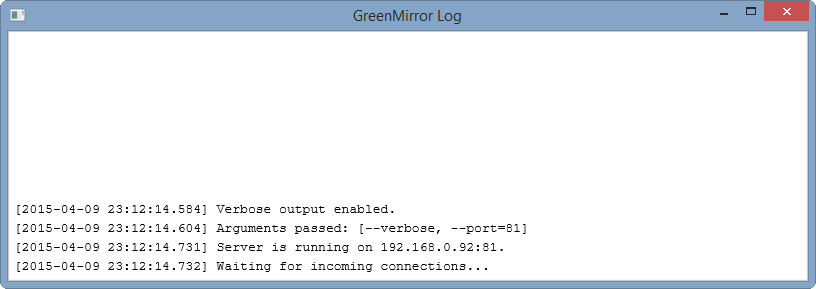
\includegraphics[width=0.95\textwidth]{images/log}
  \caption{an instance of \lstinline{WindowLogger} right after the server has been executed}
  \label{fig:log}
\end{figure}
%--------------------------------------------------------------------------------
\subsection{The \texttt{GridBuilder} class}\label{sec:features;sub:gridbuilder}
\begin{wrapfigure}{o}{0.25\textwidth}\vspace{-22pt}
  \begin{center}
    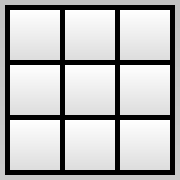
\includegraphics[width=0.23\textwidth]{images/grid}
  \end{center}
  \vspace{-10pt}\caption{the result of the \lstinline{GridBuilder} example code of \cref{lst:gridbuilder}}\vspace{-20pt}
  \label{fig:grid}
\end{wrapfigure}
GreenMirror has an auxiliary \lstinline{GridBuilder} class created to take away the tedious work of building a grid of nodes. It supports properties such as the amount of cells, the cell width and height, cell spacing, cell colour, borders, a background colour and the type and name prefix for every GreenMirror node it creates. It builds the grid by creating one GreenMirror node per cell and one for the background, all of which have the rectangle FX type. \Cref{lst:gridbuilder} shows an example of how short the code is to create a TicTacToe grid, in contrast to defining every single GreenMirror node, not to mention the tedious work of getting their exact positioning right. Doing the same without the \lstinline{GridBuilder} class takes roughly 30 lines of sloppy code. The result of \cref{lst:gridbuilder} is visible in \cref{fig:grid}.
\begin{lstlisting}[label={lst:gridbuilder}, caption={example code the user can use to build a grid of nodes}]
new GridBuilder("ticTacToeGrid:cell_")
    .setCellCount(3, 3)
    .setCellSize(50, 50)
    .setCellFill("linear-gradient(to bottom, #FFF, #DDD)")
    .setCellSpacing(5)
    .setBorderSize(5) // top, right, bottom and left
    .setBackgroundFill("black")
    .build(10, 10) // Coordinates on the visualizer
    .getNodes()
\end{lstlisting}